\documentclass[10pt]{article}
\usepackage[margin=1in]{geometry}
\usepackage[T1]{fontenc}
\usepackage{lmodern}
\usepackage{microtype}
\usepackage{amsmath,amssymb}
\usepackage{booktabs}
\usepackage{tikz}
\usepackage[numbers,sort&compress]{natbib}
\usepackage[hidelinks]{hyperref}

\newcommand{\code}[1]{\texttt{#1}}
\setlength{\emergencystretch}{3em}
\renewcommand{\bibfont}{\small}

\title{Byte-Interval Mediation: Read-Receipt Write Admission\\for Concurrent LLM Coding Agents}
\author{Joshua Pinckard\\ToolsEnabled\\\texttt{josh@toolsenabled.ai}}
\date{September 2026}

\begin{document}
\maketitle

\begin{abstract}
When several autonomous coding agents edit one working tree, each writes from its own view of files that others may have changed. The result is the lost update and the stale read of the database literature, arising in plain files with no transaction manager. We describe byte-interval mediation, the file-level concurrency control implemented as the byte authority of the ToolsEnabled engine. The authority records a durable receipt for every mediated read, binding a transport scope, a file, an exact half-open byte interval, content and file hashes, a version and a durable sequence number. It admits a patch only when the patching scope observed the changed span and every observation in its read set, on every file, still matches the bytes on disk. Length-changing edits rebase byte-disjoint observations and invalidate overlapping ones. An unmediated change forces a whole-file reread, and a whole-file write is recorded as blind replacement. Creation is exclusive, and every publication is journaled as PREPARED and then COMMITTED, so that after a crash each pending publication resolves from the bytes actually present. The implementation passes its 68 unit, recovery and multi-process tests in a standalone extraction, and 117 tests including transport integration in the engine. Six design probes pin its limits. The most important is that byte-disjoint edits can jointly break a shared invariant. In the one deployment we report, the authority was dormant, because agents wrote through host file tools that it did not mediate.
\end{abstract}

\section{Introduction}

Coding agents built on large language models now resolve repository issues end to end~\citep{jimenez2024swebench,yang2024sweagent,wang2025openhands,xia2024agentless,zhang2024autocoderover}, and frameworks run several of them together~\citep{hong2024metagpt,qian2024chatdev,wu2023autogen}. When agents share one working tree, each edits from its own view of files that others may have changed since. Two failures follow. In a \emph{lost update}, agent~B overwrites a region that agent~A changed after B read it. In a \emph{stale read}, A's edit is correct against bytes that no longer exist, possibly in another file. Both are classic isolation anomalies~\citep{berenson1995critique,adya1999weak}. Here they occur in plain files, with no transaction manager, between a read and a write that can be minutes apart while a model reasons.

This paper describes byte-interval mediation, implemented as the byte authority of the ToolsEnabled engine. Its contributions are:
\begin{enumerate}
\item a write-admission rule for files based on durable read receipts over exact byte intervals: a patch publishes only if its scope observed the changed span and everything the scope read is still current (Section~\ref{sec:design});
\item coordinate maintenance under length-changing edits, a whole-file-reread rule for unmediated changes, and an explicit class for blind whole-file writes (Section~\ref{sec:design});
\item a publication journal with exclusive, identity-checked creation, and recovery that resolves each pending publication from the bytes on disk (Sections~\ref{sec:design} and~\ref{sec:invariants});
\item a standalone extraction with the unchanged implementation and suites, six design probes that pin its limits, and an account of a deployment in which it was dormant (Sections~\ref{sec:eval} and~\ref{sec:deploy}).
\end{enumerate}
The rule does not address semantic conflicts. Two byte-disjoint edits can jointly break an invariant, and the authority admits both (probe P4, Section~\ref{sec:eval}).

\section{Setting}\label{sec:setting}

A host runs several agents. Each agent reaches files only through tools, and the host gives each authenticated tool session a private \emph{scope} that tool arguments cannot name or forge. An agent reads parts of files, reasons, and then either patches a file (replacing one exact span) or writes a whole file. Nothing orders these steps across agents.

Three design choices shape the mechanism; they are design statements, not measured results.
\emph{Validate, do not lock.} Holding locks across model inference would serialize agents for minutes and require timeouts. Instead the read set is accumulated from the reads an agent actually makes and validated when it writes, as in optimistic concurrency control~\citep{kung1981optimistic}. Observations expire, as leases do~\citep{gray1989leases}.
\emph{Refuse, do not merge.} Merging concurrent edits yields a converged file but does not tell an agent that its premise changed. A refused write returns the regions to reread, and the agent reconciles.
\emph{Bytes, not lines.} Offsets count bytes and hashes cover the exact materialized bytes, so line-ending and encoding differences cannot hide a change, and no parser is needed for any language.

\section{Design}\label{sec:design}

\paragraph{Receipts and observations.}
A \emph{resource} is a canonical absolute path to a file of at most 512\,KiB. The authority records its version, SHA-256, length and presence; a missing file and an empty file are distinct states. A read of the half-open interval $[a,b)$ materializes the whole file through an adapter, validates the window (the engine refuses windows that are not complete UTF-8) and, before releasing any content, durably records a \emph{receipt}: the scope, the resource, $[a,b)$, the SHA-256 of the returned bytes and of the whole file, the resource version, a lease expiry and the sequence number of an append-only event. The live projection of a receipt is one or more \emph{observations}: intervals with their observed bytes and an optional stale reason. A new read replaces the scope's older observations that it intersects or covers, keeping their parts outside the new window.

\paragraph{Conflict is interval intersection.}
Non-empty intervals $[a,b)$ and $[c,d)$ conflict when $a<d$ and $c<b$, so adjacent intervals do not conflict. A point $p$ (an insertion, or an observation of an empty file) conflicts with $[c,d)$ when $c \le p < d$: inserting at the left edge of another scope's observation conflicts with it, and inserting at its right edge does not. Two points conflict when they are equal.

\paragraph{Admission.}
A patch arrives as a callback that derives $[s,e)$ and replacement bytes $x$ from the current file. It is admitted only if (i) every observation of the scope, on every file, is unexpired and byte-equal to the current contents, and every file it names still exists; and (ii) the valid observations of a single receipt of the scope cover $[s,e)$. Failing (i) refuses with the list of regions to reread and no file content; failing (ii) refuses with a read-required code.

\paragraph{Rebase.}
Committing a patch with $\delta = |x| - (e - s)$ transforms every observation of the resource (Figure~\ref{fig:rebase}). An observation that does not conflict with $[s,e)$ shifts by $\delta$ if it starts at or after $e$, and is otherwise unchanged. A conflicting observation splits into its left part $[a,s)$ and its shifted right part $[e+\delta,\,b+\delta)$, both still valid, and a middle $[s,\,s+|x|)$. The middle is marked stale for other scopes; for the writing scope it becomes an observation of $x$. For eight lockfile names (for example \code{package-lock.json} and \code{cargo.lock}), any patch invalidates every other scope's observations of the file, which then need a whole-file reread.

\begin{figure}[t]
\centering
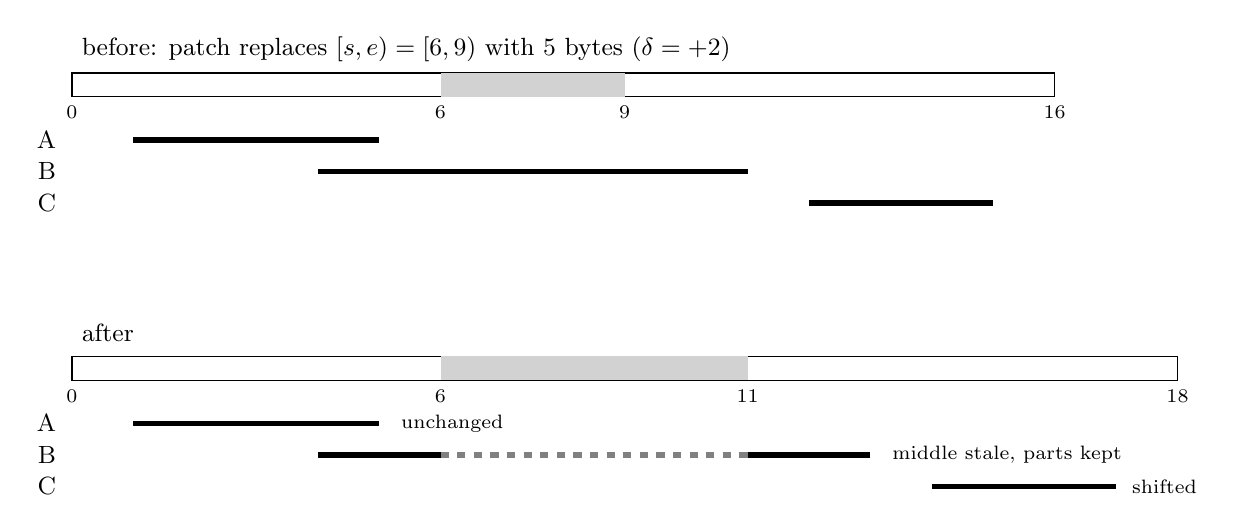
\begin{tikzpicture}[x=0.78cm,y=0.5cm,font=\small]
  \node[anchor=west] at (0,4.3) {before: patch replaces $[s,e)=[6,9)$ with 5 bytes ($\delta=+2$)};
  \draw (0,3.1) rectangle (16,3.7); \fill[gray!35] (6,3.1) rectangle (9,3.7);
  \foreach \x in {0,6,9,16} \node[below] at (\x,3.1) {\scriptsize\x};
  \node[anchor=east] at (-0.1,2.0) {A}; \draw[line width=2pt] (1,2.0) -- (5,2.0);
  \node[anchor=east] at (-0.1,1.2) {B}; \draw[line width=2pt] (4,1.2) -- (11,1.2);
  \node[anchor=east] at (-0.1,0.4) {C}; \draw[line width=2pt] (12,0.4) -- (15,0.4);
  \begin{scope}[yshift=-3.6cm]
  \node[anchor=west] at (0,4.3) {after};
  \draw (0,3.1) rectangle (18,3.7); \fill[gray!35] (6,3.1) rectangle (11,3.7);
  \foreach \x in {0,6,11,18} \node[below] at (\x,3.1) {\scriptsize\x};
  \node[anchor=east] at (-0.1,2.0) {A}; \draw[line width=2pt] (1,2.0) -- (5,2.0);
  \node[anchor=west] at (5.2,2.0) {\scriptsize unchanged};
  \node[anchor=east] at (-0.1,1.2) {B}; \draw[line width=2pt] (4,1.2) -- (6,1.2);
  \draw[line width=2pt,dashed,gray] (6,1.2) -- (11,1.2); \draw[line width=2pt] (11,1.2) -- (13,1.2);
  \node[anchor=west] at (13.2,1.2) {\scriptsize middle stale, parts kept};
  \node[anchor=east] at (-0.1,0.4) {C}; \draw[line width=2pt] (14,0.4) -- (17,0.4);
  \node[anchor=west] at (17.1,0.4) {\scriptsize shifted};
  \end{scope}
\end{tikzpicture}
\caption{Rebase of three other scopes' observations when a patch replaces $[6,9)$ with five bytes. Solid: valid; dashed: stale, reread required.}
\label{fig:rebase}
\end{figure}

\paragraph{Unmediated changes and blind writes.}
Whenever the authority materializes a resource whose presence, hash or length differs from its record, it increments the version and marks every observation of the resource stale. No coordinate transform is known for such a change, so only a whole-file read clears it. A whole-file write is \emph{blind replacement}: it needs no read of its target and creates none, not even for the writer, though the writer's read set is still validated. Once committed, it invalidates every observation of the resource, the writer's included.

\paragraph{Leases.}
An observation lasts 60 minutes. When another scope holds a live observation of the same resource, a new one lasts 60 seconds, and every observation of that resource is capped at 60 seconds. An expired observation must be reread.

\paragraph{Publication, creation and recovery.}
Every operation runs inside one \emph{lifetime lock}: an SQLite \code{BEGIN IMMEDIATE} transaction on a dedicated lock database~\citep{sqlite-locking,sqlite-transaction}, held for the whole asynchronous operation. The operating system releases it if the holder dies, and nothing steals it by age. State lives in a second database with full synchronous commits, so a PREPARED record, carrying a SHA-256 checksum over the operation, is durable before publication while the lock is still held. The publisher replaces the file by rename~\citep{posix2024rename} and receives a synchronous scope check to run immediately before it. The authority then re-materializes the file, confirms the after-image, and in one transaction applies the rebase or invalidation, increments the version and marks the operation COMMITTED. If the scope is revoked after commit, the call reports that the write committed, never that it was refused. Creating a missing file writes an exclusively created, fsynced sibling stage whose device, inode, digest and length are journaled in PREPARED, and publishes it by hard link, which fails rather than replace a file that appeared meanwhile~\citep{posix2024link}. Recovery runs before every admission, for the target and for every resource the scope has read. It validates each pending operation's checksum, fields, scope and base version, then lets the bytes decide: the before-image marks it ABORTED, and the after-image (with the staged identity, for a creation) marks it COMMITTED with its effects applied. Any other state marks it UNKNOWN, which blocks the resource and the scopes that read it, but not unrelated work. A missing or corrupt store refuses; it is never treated as empty history.

\section{Invariants}\label{sec:invariants}

Write $F_r$ for the current bytes of resource $r$ and $F_r[a{:}b]$ for a slice. An observation is $o=\langle\sigma,r,[a,b),\beta,\tau,\kappa\rangle$: scope, resource, interval, observed bytes, expiry and stale reason ($\kappa=\bot$ if none). It is \emph{valid} at time $t$ when
\[
\mathrm{valid}(o,t) \iff \kappa=\bot \,\wedge\, \tau>t \,\wedge\, b\le|F_r| \,\wedge\, F_r[a{:}b]=\beta .
\]
The following hold by construction of the code paths named in Section~\ref{sec:design}, assuming correct adapters and SQLite's transactional atomicity.

\begin{description}
\item[I1 Receipts.] A receipt for $[a,b)$ of $r$ at version $v$ records $H(F_r[a{:}b])$ and $H(F_r)$ as materialized at $v$, and is durable before the bytes are released.
\item[I2 Admission.] A patch of $[s,e)$ by $\sigma$ commits at $t$ only if every observation of $\sigma$ is valid at $t$, and the valid observations of one receipt of $\sigma$ on $r$ cover $[s,e)$.
\item[I3 Invalidation.] Committing a write marks stale every other scope's observation that conflicts with its span (for a whole-file write, every observation of the resource), in the same transaction that marks the operation COMMITTED.
\item[I4 Drift.] If a materialization of $r$ differs from the recorded presence, hash or length, the version of $r$ increases and every observation of $r$ becomes stale until a whole-file read.
\item[I5 Journal.] PREPARED is durable before publication. COMMITTED implies the after-image, and for a creation the staged identity, was confirmed on disk. Recovery moves PREPARED only to ABORTED on the before-image, to COMMITTED on the after-image, or to UNKNOWN otherwise. An operation's read-set effects and version increment are applied exactly when it becomes COMMITTED.
\end{description}

\paragraph{Proposition (no lost update between mediated patches).}
\emph{If every write to $r$ is mediated, a committed patch never overwrites a byte whose latest write its scope did not observe.}
Sketch. Let patch $P$ by $\sigma$ replace $[s,e)$. By I2, valid observations of $\sigma$ cover $[s,e)$, so $F_r[s{:}e]$ equals what $\sigma$ observed. Suppose a write $W$ by another scope changed a byte in $[s,e)$ after $\sigma$ observed it. By I3, $W$'s commit marked $\sigma$'s conflicting observation stale, which contradicts validity. So $\sigma$ must have reread after $W$, and the byte's latest write is one it observed. Bytes outside $[s,e)$ are untouched, and their observations are shifted, not invalidated. An unmediated change before $P$'s admission is caught by I4, because admission materializes $r$. A change between the publisher's final comparison and its rename is outside the proposition's assumption.

The same argument, applied to observations on other files, gives read-set freshness. A write by $\sigma$ on any file commits only if nothing $\sigma$ observed anywhere has changed since, which covers cross-file stale reads such as an edit made against an interface that has since moved. These are sketches of the mechanism, not machine-checked proofs.

\section{Implementation}\label{sec:impl}

The authority is one 875-line CommonJS module for Node.js~22. It uses the built-in \code{node:sqlite} module~\citep{nodejs-sqlite}, which Node still labels experimental; the warning appears in our logs. The data store has seven tables (metadata, scopes, resources, receipts, observations, operations and an append-only event log) at schema version~2, with an in-place migration from version~1 that preserves version-1 journal records and their checksums byte for byte. Refusals carry typed codes and repair lists but never file content. Callers supply four adapters: \code{materialize}, \code{publish}, and \code{prepareCreate} and \code{reconcileCreateStage} for creation.

In the engine, the authority backs the \code{repo.read\_file}, \code{repo.write\_file} and \code{repo.patch\_file} tools and the paired-desktop \code{workspace.read}. The engine's adapters read through a descriptor opened with \code{O\_NOFOLLOW}, bounded in size, and compare device, inode, size and timestamps before and after the read. They refuse symbolic-link and hard-link aliases. On publication they compare the before-image, write and fsync a temporary, compare the before-image again, and rename under a whole-file lock. \code{repo.patch\_file} derives its span as the unique occurrence of the caller's old text in the current bytes. Each tool call also receives a one-shot invocation capability, and paired-desktop scopes are revoked on disconnect, timeout, key rotation and shutdown.

The standalone extraction keeps the engine's directory layout. The authority, its five suites and their three helper files are byte-identical to the engine (git blob hashes are listed in the repository). The two modules the authority requires are replaced by POSIX stand-ins: path admission reduces to the engine's POSIX behavior, an absolute-path check and normalization, and the default state directory follows XDG conventions. Windows account confinement is not extracted, and the stand-in refuses to run on Windows.

\section{Evaluation}\label{sec:eval}

\paragraph{Test suites.}
Table~\ref{tab:suites} lists every suite. The five core suites exercise the authority through real SQLite databases and real files. The operations include two concurrent operating-system processes making disjoint edits with shifted coordinates, a competing process blocked on the held lock, and process exit before publication, after publication and between link and unlink. They also include injected publisher failures, deleted and corrupted stores, revocation in an asynchronous gap, racing creators, extra hard-link aliases, equal-content file substitution, and version-1 migration. The three transport suites run only in the engine; they exercise its tool registry, MCP dispatch and paired-desktop transport. All results come from one file per process. Standalone runs used Node.js~22.19.0 on Linux x64.

\begin{table}[t]
\centering\small
\begin{tabular}{@{}lrrp{5.6cm}@{}}
\toprule
Suite & Standalone & Engine & Exercises \\
 & 2026-09-11 & \code{c34cab8c} & \\
\midrule
\code{byte-authority} & 17/17 & 17/17 & receipts, admission, rebase, leases, lockfiles, revocation \\
\code{byte-authority-recovery} & 8/8 & 8/8 & failed publication, quarantine, store loss and corruption \\
\code{byte-authority-process} & 10/10 & 10/10 & real processes: contention, exit at crash points \\
\code{byte-authority-write} & 15/15 & 15/15 & blind writes, creation, dependencies, final guards \\
\code{byte-authority-write-recovery} & 18/18 & 18/18 & creation recovery, identity checks, migration \\
\code{repo-byte-transport} & -- & 27/27 & registry and MCP dispatch, text encodings \\
\code{remote-byte-scope} & -- & 10/10 & paired-desktop scopes and revocation \\
\code{fra-byte-mediation} & -- & 12/12 & remote workspace reads through the same authority \\
\midrule
Total & 68/68 & 117/117 & \\
\bottomrule
\end{tabular}
\caption{Passing tests over tests run, one file per process. Engine runs are at engine commit \code{c34cab8c}, whose authority and suites are byte-identical to the extraction. Sources: \code{data/standalone/}, \code{data/engine-runs/}, \code{data/results.csv}.}
\label{tab:suites}
\end{table}

\paragraph{Design probes.}
A design review wrote seven probes against the engine, and six of them concern the authority (Table~\ref{tab:probes}). A probe passes when the limitation it names is reproduced. Each passed against the engine on 2026-09-07 and again in the standalone extraction. The probes are constructed demonstrations of mechanism; they say nothing about how often these cases arise in practice.

\begin{table}[t]
\centering\small
\begin{tabular}{@{}llp{9.2cm}@{}}
\toprule
Probe & Class & Reproduced behavior \\
\midrule
P1 & liveness & A deleted file in a scope's read set blocks that scope's later write to an unrelated file. \\
P2 & liveness & A second reader caps an unchanged observation's lease at 60\,s; after it lapses the first reader must reread. \\
P3 & lost update & A blind whole-file write of bytes read outside mediation erases a peer's committed patch. \\
P4 & semantics & Two byte-disjoint patches turn ``1,1'' into ``0,0''; both commit. \\
P5 & identity & A new scope has no predecessor read set, so a resumed agent's carried-over context is unchecked. \\
P7 & retention & A committed whole-file payload is still in the store after its scope closes. \\
\bottomrule
\end{tabular}
\caption{Design probes. P6 of the original set tested an unrelated module and is omitted. Sources: \code{probes/}, \code{data/standalone/design-probes.tap}, \code{data/engine-runs/2026-09-07/design-probes.tap}.}
\label{tab:probes}
\end{table}

\paragraph{Not measured.}
We did not measure latency or throughput, refusal or conflict rates with real agents, whether agents reconcile correctly after a refusal, durability under power loss, or behavior on Windows. The authority serializes every operation through one cross-process transaction, and its many-agent throughput is unknown.

\section{Deployment experience}\label{sec:deploy}

In ToolsEnabled 1.0.44 (engine package 1.4.0), the authority was wired to the \code{repo.*} tools and the paired-desktop read path. The \code{repo.*} tools resolve paths against the engine's own package root. In an installed build that root is the installed payload, and generic writes into it are refused. The agents in that deployment edited their working clones through \code{host.read\_file}, \code{host.write\_file} and \code{host.exec}. The host file provider takes a whole-file write lock and records an audit entry, but never consults the authority. The authority was therefore effectively dormant. It produced no production conflict data, and we report none. A mediation layer protects only the write paths routed through it, and the paths these agents used were not.

Mediation of \code{host.read\_file}, \code{host.write\_file} and a new \code{host.patch\_file} through the same authority is being implemented at the time of writing. It uses a store namespace separate from \code{repo.*}, prunes committed payloads, and adds an off switch. Unlike \code{repo.write\_file}, \code{host.write\_file} is designed to replace an existing file only when the writing scope currently observes all of it, which would close P3 for host files. Its receipt had no test verdict when this paper was written, so we report only two preliminary measurements from its branch (\code{data/host-mediation-preliminary/}), taken on a machine that was running other work. First, over 100 interleaved iterations on a 100\,KB file, a \code{host.read\_file} plus \code{host.write\_file} round trip through the engine's tool dispatcher took 266.01\,ms at the median and 334.26\,ms at the 95th percentile with mediation, against 213.73\,ms and 266.01\,ms without it. Second, over 500 writes of 100\,KB, the host store grew by 141,148,160 bytes when committed payloads were kept and by 4,931,584 bytes when they were pruned at commit.

\section{Related work}\label{sec:related}

\paragraph{Concurrency control and isolation.}
Optimistic concurrency control records a transaction's read set during execution and validates it at commit~\citep{kung1981optimistic}. The authority applies that rule to file bytes, with the read set built from mediated tool calls. Predicate locks~\citep{eswaran1976notions} protect sets defined by conditions; byte intervals are range predicates over offsets, used here for validation rather than locking. The lost update, read skew and write skew are characterized by \citet{berenson1995critique}, generalized by \citet{adya1999weak}, and addressed for snapshot isolation by \citet{fekete2005making}. Leases bound how long cached state may be trusted~\citep{gray1989leases}, as observation expiry does here.

\paragraph{Conditional requests.}
HTTP makes a write conditional on a validator such as an entity tag through \code{If-Match}~\citep{rfc9110}. A server can require such preconditions with status 428~\citep{rfc6585}, and ETags with unreserved checkout were proposed specifically against the lost update in web authoring~\citep{w3c1999lostupdate}. Byte-interval mediation is a conditional write whose precondition is the writer's whole read set at byte granularity. The server records the read set as reads happen, instead of trusting a validator presented by the client.

\paragraph{Operational transformation, CRDTs and merging.}
Operational transformation rewrites concurrent operations so that replicas converge~\citep{ellis1989concurrency,sun1998achieving}. CRDTs converge by construction~\citep{shapiro2011crdt,kleppmann2017json}. Three-way merge integrates divergent versions after the fact~\citep{khanna2007diff3,mens2002merging}. Rebase is a position transform of the same kind as in operational transformation, applied to read intervals rather than to operations. Where intervals conflict, the authority refuses instead of transforming, because an agent's premise, not only its text, may have changed. Conflicts that survive a clean textual merge are studied by \citet{brun2011proactive}, and \citet{sousa2018verified} verify semantic conflict freedom of merges. Probe P4 is such a conflict.

\paragraph{Intent logging and crash consistency.}
Write-ahead logging with redo and undo is the foundation of transactional recovery~\citep{mohan1992aries}. Application-level crash consistency on file systems depends on fsync and rename behavior that applications often get wrong~\citep{pillai2014allfs}. The authority's journal is an intent log for a single file publication, and recovery decides between redo and abort by comparing the bytes on disk with the journaled before-image and after-image.

\paragraph{Agents and change impact.}
Work on LLM software engineering, from benchmarks to agent systems~\citep{jimenez2024swebench,yang2024sweagent,wang2025openhands,xia2024agentless,zhang2024autocoderover}, mostly evaluates one agent working on a repository at a time. Multi-agent frameworks~\citep{hong2024metagpt,qian2024chatdev,wu2023autogen} organize agents by roles, conversations and hand-offs, and a taxonomy of multi-agent failures~\citep{cemri2025multiagent} includes coordination breakdowns. This paper concerns the layer below: what happens when two agents' edits to the same file interleave. Three recent preprints address that layer directly. CooperBench evaluates coding agents that must coordinate separate features in one repository~\citep{khatua2026cooperbench}. STORM mediates agents' interactions with a shared workspace, so that each works on a consistent view and conflicting edits are detected and resolved at write time~\citep{liu2026storm}. CoAgent argues that locks block long inference and that optimistic abort-and-retry discards work. It fixes a serialization order at launch, applies writes speculatively in place, and has affected agents repair their plans~\citep{lyu2026coagent}. Byte-interval mediation refuses a stale write and names the regions to reread, which leaves reconciliation to the agent; we have not measured what that costs in agent work. Co-change mining predicts which files change together~\citep{zimmermann2005mining}. The companion Blast-Radius project~\citep{pinckard2026blastradius} designs an estimator for which regions a change may invalidate where no read was recorded. Byte-interval mediation is the exact tier beneath that estimator: where a read was recorded, the answer is a lookup.

\section{Limitations and future work}\label{sec:limits}

\begin{itemize}
\item \textbf{Semantic dependence.} Receipts show what was read, not what the work depends on (P4). A next step is \emph{semantic dependency witnesses}: evidence recorded beside receipts, such as tests executed, symbols resolved or contracts consulted, against which a write can be checked.
\item \textbf{Coverage.} Unmediated writers are detected only when next observed, and a change landing between the final comparison and the rename is not caught. Mediation of the host file tools is the ongoing work described in Section~\ref{sec:deploy}.
\item \textbf{Blind writes} of bytes obtained outside mediation can erase a peer's patch (P3).
\item \textbf{Scope continuity.} Scopes are not bound to launch, lane or run records, so a resumed agent does not inherit or revalidate its predecessor's read set (P5).
\item \textbf{Liveness.} A deleted dependency blocks its scope until the file is restored and reread (P1), and contention cuts leases to 60 seconds (P2). The repair budget with escalation that the design specified is not built.
\item \textbf{Retention.} Committed payloads are never pruned (P7).
\item \textbf{Scale and platform.} There is a 512\,KiB limit per file and a single serializing transaction. Throughput is unmeasured, recovery covers process crashes rather than power loss, and the extraction runs on POSIX only.
\end{itemize}

\section*{Author contributions and AI assistance}
Joshua Pinckard conceived the project, defined its objectives and requirements, directed the autonomous agent workflows, selected and evaluated outputs, and assumes responsibility for the research methodology and conclusions. AI agents generated substantial portions of the implementation and written drafts.

\section*{Availability}
Code, tests, probes and data: \url{https://github.com/JoshuaPinckard/byte-interval-mediation}, MIT License.

\bibliographystyle{plainnat}
\bibliography{refs}

\end{document}
